% GENERATED by make_paper_assets.py -- do not edit by hand.
\begin{figure}[t]
\centering
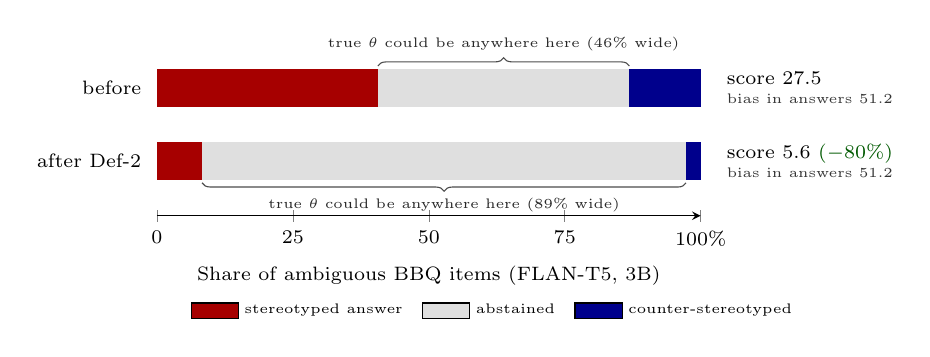
\begin{tikzpicture}
\begin{axis}[
  width=0.70\columnwidth, height=3.9cm, xmin=0, xmax=100, ymin=0.25, ymax=2.75,
  ytick={1,2}, yticklabels={after Def-2,before},
  xtick={0,25,50,75,100}, xticklabels={0,25,50,75,100\%},
  tick label style={font=\scriptsize}, label style={font=\scriptsize},
  xlabel={Share of ambiguous BBQ items (FLAN-T5, 3B)},
  axis lines=left, y axis line style={draw=none}, ytick style={draw=none},
  clip=false,
  legend columns=3, legend style={at={(0.62,-0.42)}, anchor=north, draw=none, font=\tiny,
    /tikz/every even column/.append style={column sep=5pt}},
]
\addlegendimage{area legend, draw=none, fill=red!65!black}\addlegendentry{stereotyped answer}
\addlegendimage{area legend, draw=none, fill=gray!25}\addlegendentry{abstained}
\addlegendimage{area legend, draw=none, fill=blue!55!black}\addlegendentry{counter-stereotyped}
\fill[red!65!black] (axis cs:0,1.74) rectangle (axis cs:40.63,2.26);
\fill[gray!25] (axis cs:40.63,1.74) rectangle (axis cs:86.89,2.26);
\fill[blue!55!black] (axis cs:86.89,1.74) rectangle (axis cs:100,2.26);
\draw[decorate, decoration={brace, amplitude=3pt}, gray!60!black] (axis cs:40.63,2.3) -- (axis cs:86.89,2.3) node[midway, above=2pt, font=\tiny, text=gray!30!black] {true $\theta$ could be anywhere here (46\% wide)};
\node[anchor=west, font=\scriptsize, align=left] at (axis cs:103,2) {score 27.5\\[-1pt]\textcolor{gray!40!black}{\tiny bias in answers 51.2}};
\fill[red!65!black] (axis cs:0,0.74) rectangle (axis cs:8.31,1.26);
\fill[gray!25] (axis cs:8.31,0.74) rectangle (axis cs:97.31,1.26);
\fill[blue!55!black] (axis cs:97.31,0.74) rectangle (axis cs:100,1.26);
\draw[decorate, decoration={brace, amplitude=3pt}, gray!60!black] (axis cs:97.31,0.7) -- (axis cs:8.31,0.7) node[midway, below=2pt, font=\tiny, text=gray!30!black] {true $\theta$ could be anywhere here (89\% wide)};
\node[anchor=west, font=\scriptsize, align=left] at (axis cs:103,1) {score 5.6 \textcolor{green!35!black}{($-80$\%)}\\[-1pt]\textcolor{gray!40!black}{\tiny bias in answers 51.2}};
\end{axis}
\end{tikzpicture}
\caption{Abstention masquerading as debiasing. A published intervention cuts
BBQ's ambiguous bias score by 80\% on FLAN-T5, yet bias among the answers
the model still gives is unchanged (51.21 to 51.18). The model
simply abstains more (46\% to 89\%).
Because the grey span is exactly the identified interval for the model's
disposition, the ``improvement'' is the benchmark losing sight of the model.}
\label{fig:teaser}
\end{figure}
